%%%%%%%% ICML 2021 EXAMPLE LATEX SUBMISSION FILE %%%%%%%%%%%%%%%%%

\documentclass{article}

% Recommended, but optional, packages for figures and better typesetting:
\usepackage{microtype}
\usepackage{graphicx}
\usepackage{subfigure}
\usepackage{booktabs} % for professional tables
\usepackage{multirow}
% hyperref makes hyperlinks in the resulting PDF.
% If your build breaks (sometimes temporarily if a hyperlink spans a page)
% please comment out the following usepackage line and replace
% \usepackage{icml2021} with \usepackage[nohyperref]{icml2021} above.
\usepackage{hyperref}

% Attempt to make hyperref and algorithmic work together better:
\newcommand{\theHalgorithm}{\arabic{algorithm}}

% Define the subsubsubsection command
\newcommand{\subsubsubsection}[1]{%
  \paragraph{#1}\mbox{}\\}





\usepackage[accepted]{icml2021}

\icmltitlerunning{Wine Quality Prediction}

\begin{document}

\twocolumn[
\icmltitle{Wine Quality Prediction}

\begin{icmlauthorlist}
\icmlauthor{Stijn de Preter (852726504)}{ou}
\icmlauthor{Arjan Broer (850166428)}{ou}
\end{icmlauthorlist}

\icmlaffiliation{ou}{Open Universiteit}
\icmlcorrespondingauthor{}{}

% You may provide any keywords that you
% find helpful for describing your paper; these are used to populate
% the "keywords" metadata in the PDF but will not be shown in the document
\icmlkeywords{wine quality, machine learning, neural networks, ANN, SVR }

\vskip 0.3in
]

\section{Brief Introduction}
The assignment is based on the article \cite{dahal2021prediction} and focuses on the reproduction of the article results.
The reproduct is limited to only the Support Vector Regression (SVR) and Artificial Neural Network (ANN) models.
The Ridge Regression (RR) and Gradient Boosting Regression models are not included in this report.
The goal of the assignment is to predict the quality of wine based on its chemical properties and understand the methods used to generate the predictions.
The dataset will be analyzed to find the features that most influence the quality of wine and suggestions are provided to improve the hyperparameters of the model for best results.

The research questions discussed in this report are:
\begin{enumerate}
    \item Reproduce the results of the article \cite{dahal2021prediction} using the same dataset and models.
    \item Analyze the dataset to find the features that most influence the quality of wine.
    \item Provide suggestions to improve the hyperparameters of the model for best results.
\end{enumerate}

\section{Methods}
Describe the methods used. How it works. It can include algorithms, system descriptions, new language constructs, analyses, etc.
Provide diagrams to help in the discussion. Figure \ref{Reproduce-SVR-the-results} and Figure \ref{fig:two-col-figure} shows an example of a one-column figure and a two-column figure. 
\begin{figure}
    \centering
    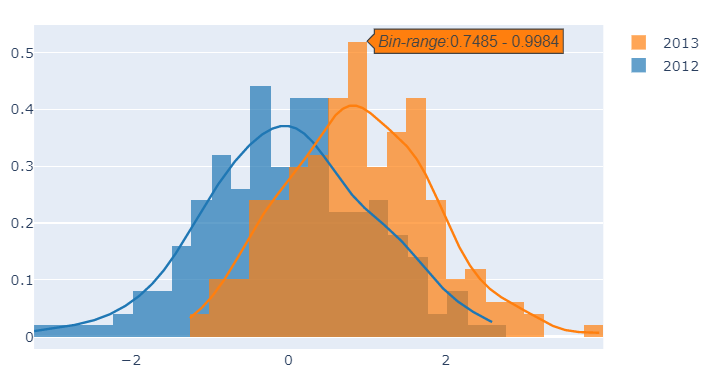
\includegraphics[width=\linewidth]{figures/example_plot.png}
    \caption{One-column figure that explains the steps or framework of your method / model.}
    \label{fig:one-col-figure}
\end{figure}

\subsection{SVR and ANN - Reproduce the results}
In order to compare the results of the article with our results, a visualization was made. Here the values of the article (\textbf{still to be added}) are compared with our results repeatedly. Our results are reproduced repeatedly with different test and training data each time. This way we are sure that it is not a lucky shot but we get a realistic picture of how our model performs.
Also, standardization has been applied to the data features of the dataset, not to the quality column.

\subsection{SVR and ANN - Impact of the features}
TBC

\subsection{SVR and ANN - Inprove the model}
For optimizing the hyperparameters, gridsearch and BayesSearch were used for SVR. For ANN, gridsearch was used to examine the impact of the hyperparameters.

\begin{figure*}
    \centering
    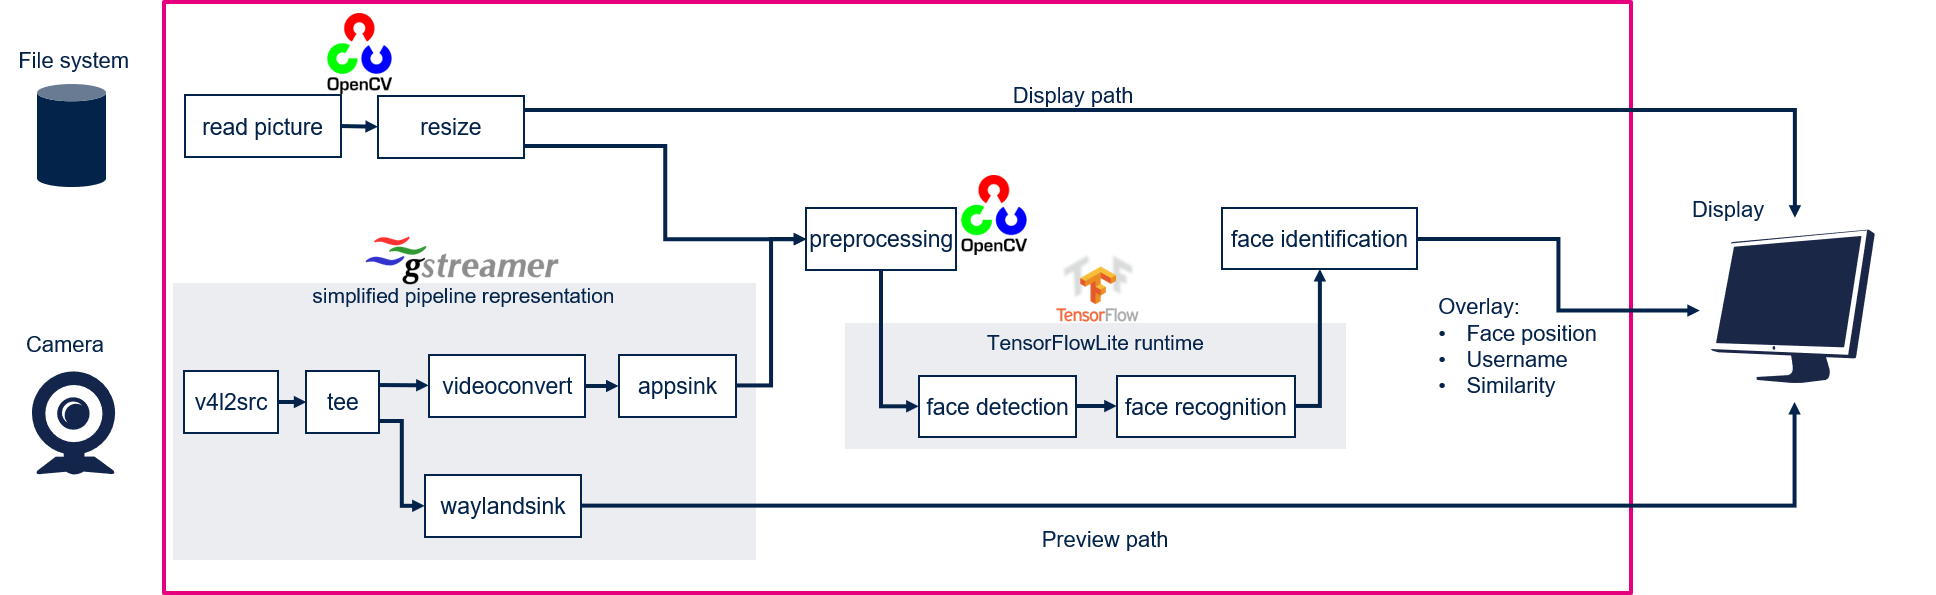
\includegraphics[width=\linewidth]{figures/example_pipeline.png}
    \caption{One-column figure that explains the steps or framework of your method / model.}
    \label{fig:two-col-figure}
\end{figure*}

\section{Experimental Results}
This chapter, experimental results, is split into 3 parts: A short general piece, a piece on SVR and a part on ANN

\subsection{Datasets}
When exploiting the data it was found that the information given in the article about the data did not match the information about the data. The article indicates that the red wine dataset was used. Based on the number of rows and other metadata (averages, Median, ...) we see that the white wine dataset was used. In the rest of this article we will work with the white wine dataset.

\subsection{SVR}

\subsubsection{Datasets}
The article indicates that the data is split into training data and testing data with a ratio of 3:1. This is also the ratio of the splits that was applied in further research.

\subsubsection{Implementation Details}

\subsubsubsection{Reproduce the results}
The results of the article are simulated by using the parameters mentioned in the article. The following parameters are mentioned: kernel=rbf, cost = 0.95 and Gamma = 0.13. For all other parameters, the default parameters of sklearn are chosen, except for the Tolerance for stopping criterion, which is set to 0.0001 to obtain the best possible result and because the cost is negligible given the small dataset.
How the training data is chosen is unknown, so the split between training and test data is performed multiple times. In this way, there is a realistic picture of the models that generate these parameters.

\subsubsubsection{Impact of the features}
tbc

\subsubsubsection{Inprove the model}
To optimize the model, the cost and gamma were examined. BayesSearch was used to find a model with the lowest possible mean squared error. 

\subsubsection{Results}

\subsubsubsection{Reproduce the results}
\begin{figure*}
\centering
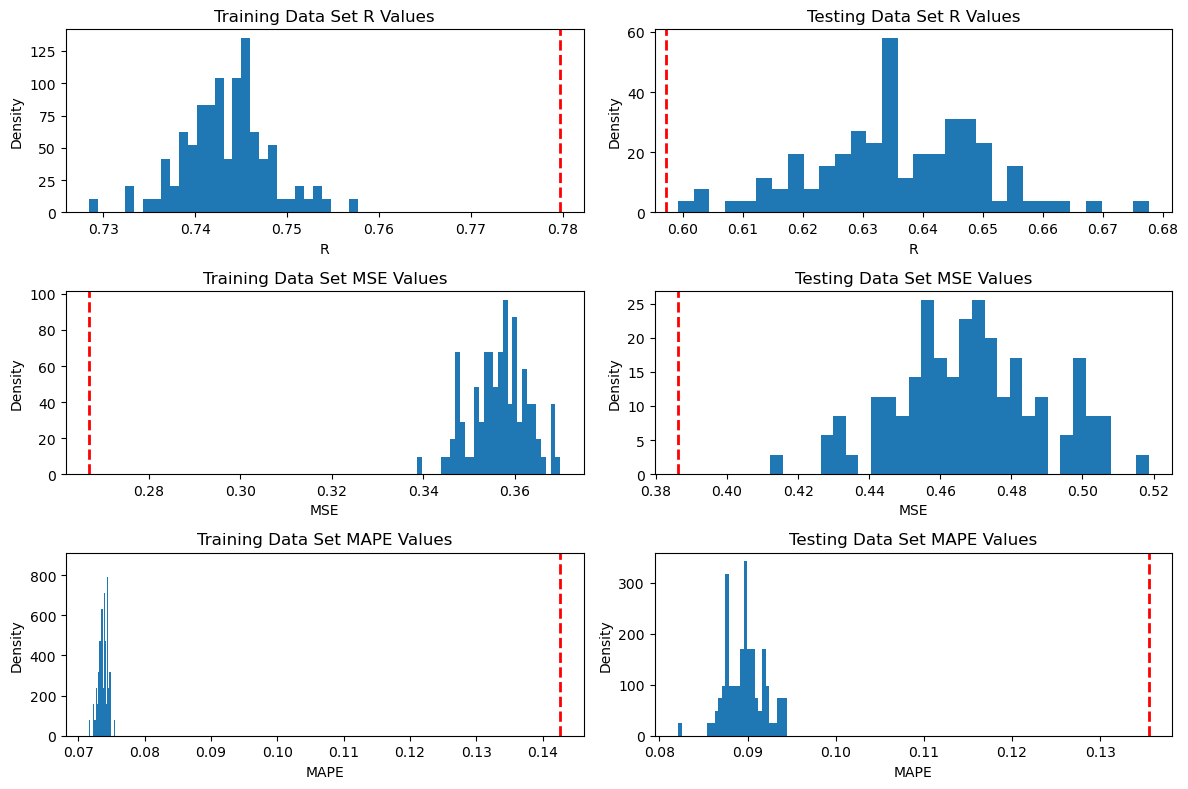
\includegraphics[width=\linewidth]{figures/SVR_reproduce_the_results.png}
\caption{Reproduce the results}
\label{fig:Reproduce-SVR-the-results}
\end{figure*}

\subsubsubsection{Impact of the features}
tbc


\subsubsubsection{Inprove the model}

In figure \ref{Reproduce-SVR-the-results}   the best possible values for gamma and cost are examined. The non-optimized model (the model with the parameters as indicated in the article) is visualized by a blue sphere.
\begin{figure*}
    \centering
    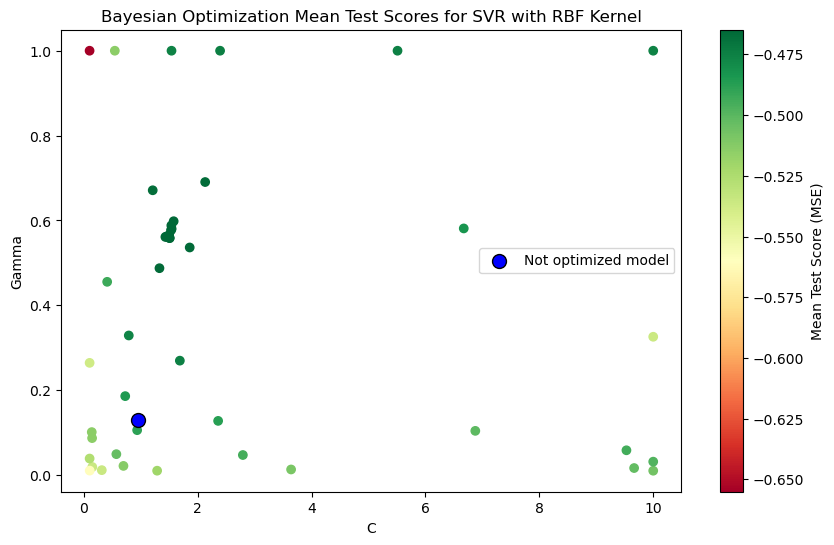
\includegraphics[width=\linewidth]{figures/bayesian_optimization.png}
    \caption{Bayesian search for optimal gamma en cost}
    \label{fig:optimized-model}
\end{figure*}

The most optimal parameters are: cost=1.51 and gamma=0.558.
In figure \ref{optimized-model} we see how the model performs compared to the values of the article model (dashed line) and compared to the non-optimized model (dotted line).
\begin{figure*}
	\centering
	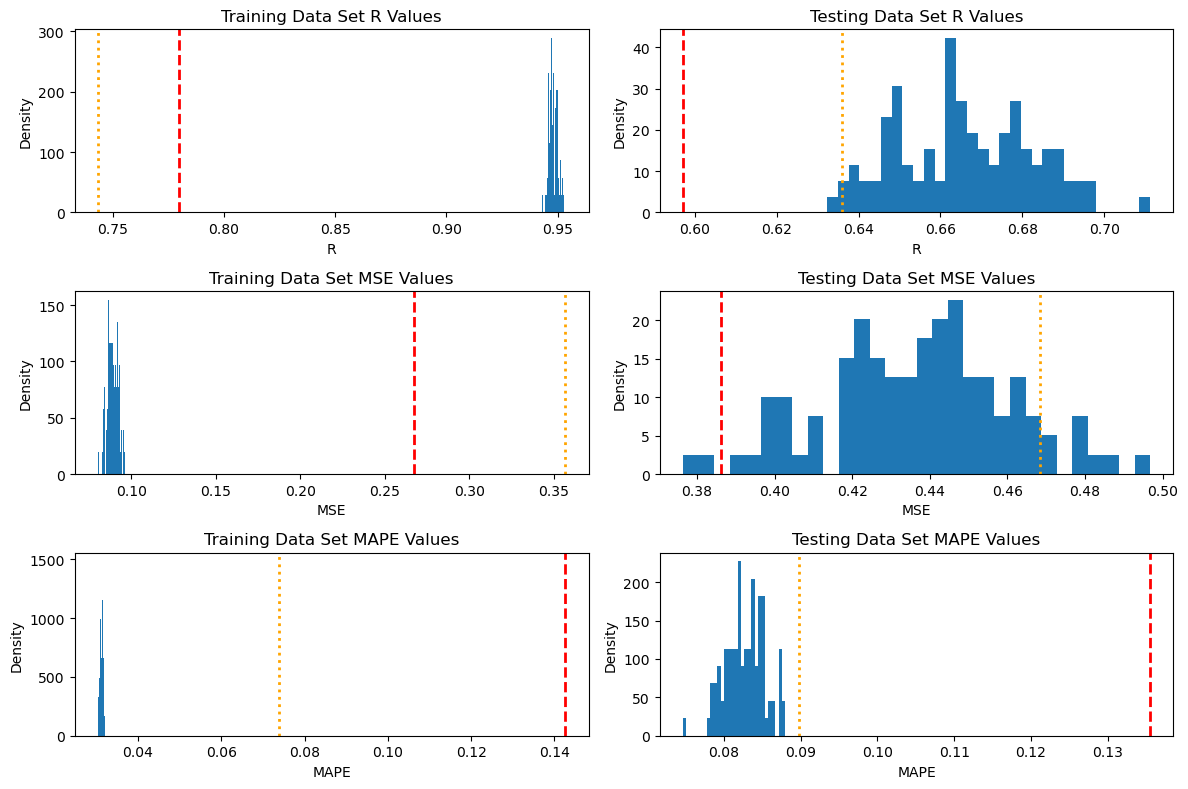
\includegraphics[width=\linewidth]{figures/SVR_optimized_model.png}
	\caption{Bayesian search for optimal gamma en cost}
	\label{fig:one-col-figure}
\end{figure*}


\subsubsection{Discussion}
%Additionally, you can include a separate discussion section in which you summarize the results, indicate possible limitations of your work, and provide suggestions for future research.


The results of the article have been reproduced. The impact of the features has been investigated. And the model has been optimized. All this while the article does not seem reliable because of the incorrect naming of the data set (namely red wine instead of white wine)


\subsection{Citing references}
LaTeX manages the citations for you. You simply have to add the bibtex entry for the reference in the references.bib file and you can use the citation in the paper \cite{langley00}. You can also cite multiple references in one command \cite{DudaHart2nd,Newell81,kearns89}. The bibtex entries for a paper can be obtained in websites such as google scholar or dblp.

\subsection{ANN}

\subsubsection{Datasets}


\subsubsection{Implementation Details}


\subsubsection{Results}


\subsubsection{Discussion}


\subsubsection{Citing references}


\bibliography{references}
\bibliographystyle{icml2021}


\end{document}

